

Fully Sharded Data Parallel (FSDP) is capable of scaling to accommodate large models that may not fit in a single GPU device by sharding the dense parameters. More specifically, FSDP decomposes the model instance into smaller units and handles each unit independently. During forward and backward computation, FSDP only materializes unsharded parameters and gradients of one unit at a time, and otherwise, it keeps parameters and gradients sharded. Throughout the training loop, the optimizer states are kept sharded. The memory requirements for FSDP are proportional to the size of the sharded model plus the size of the largest fully-materialized FSDP unit.


\begin{figure}
    \centering
    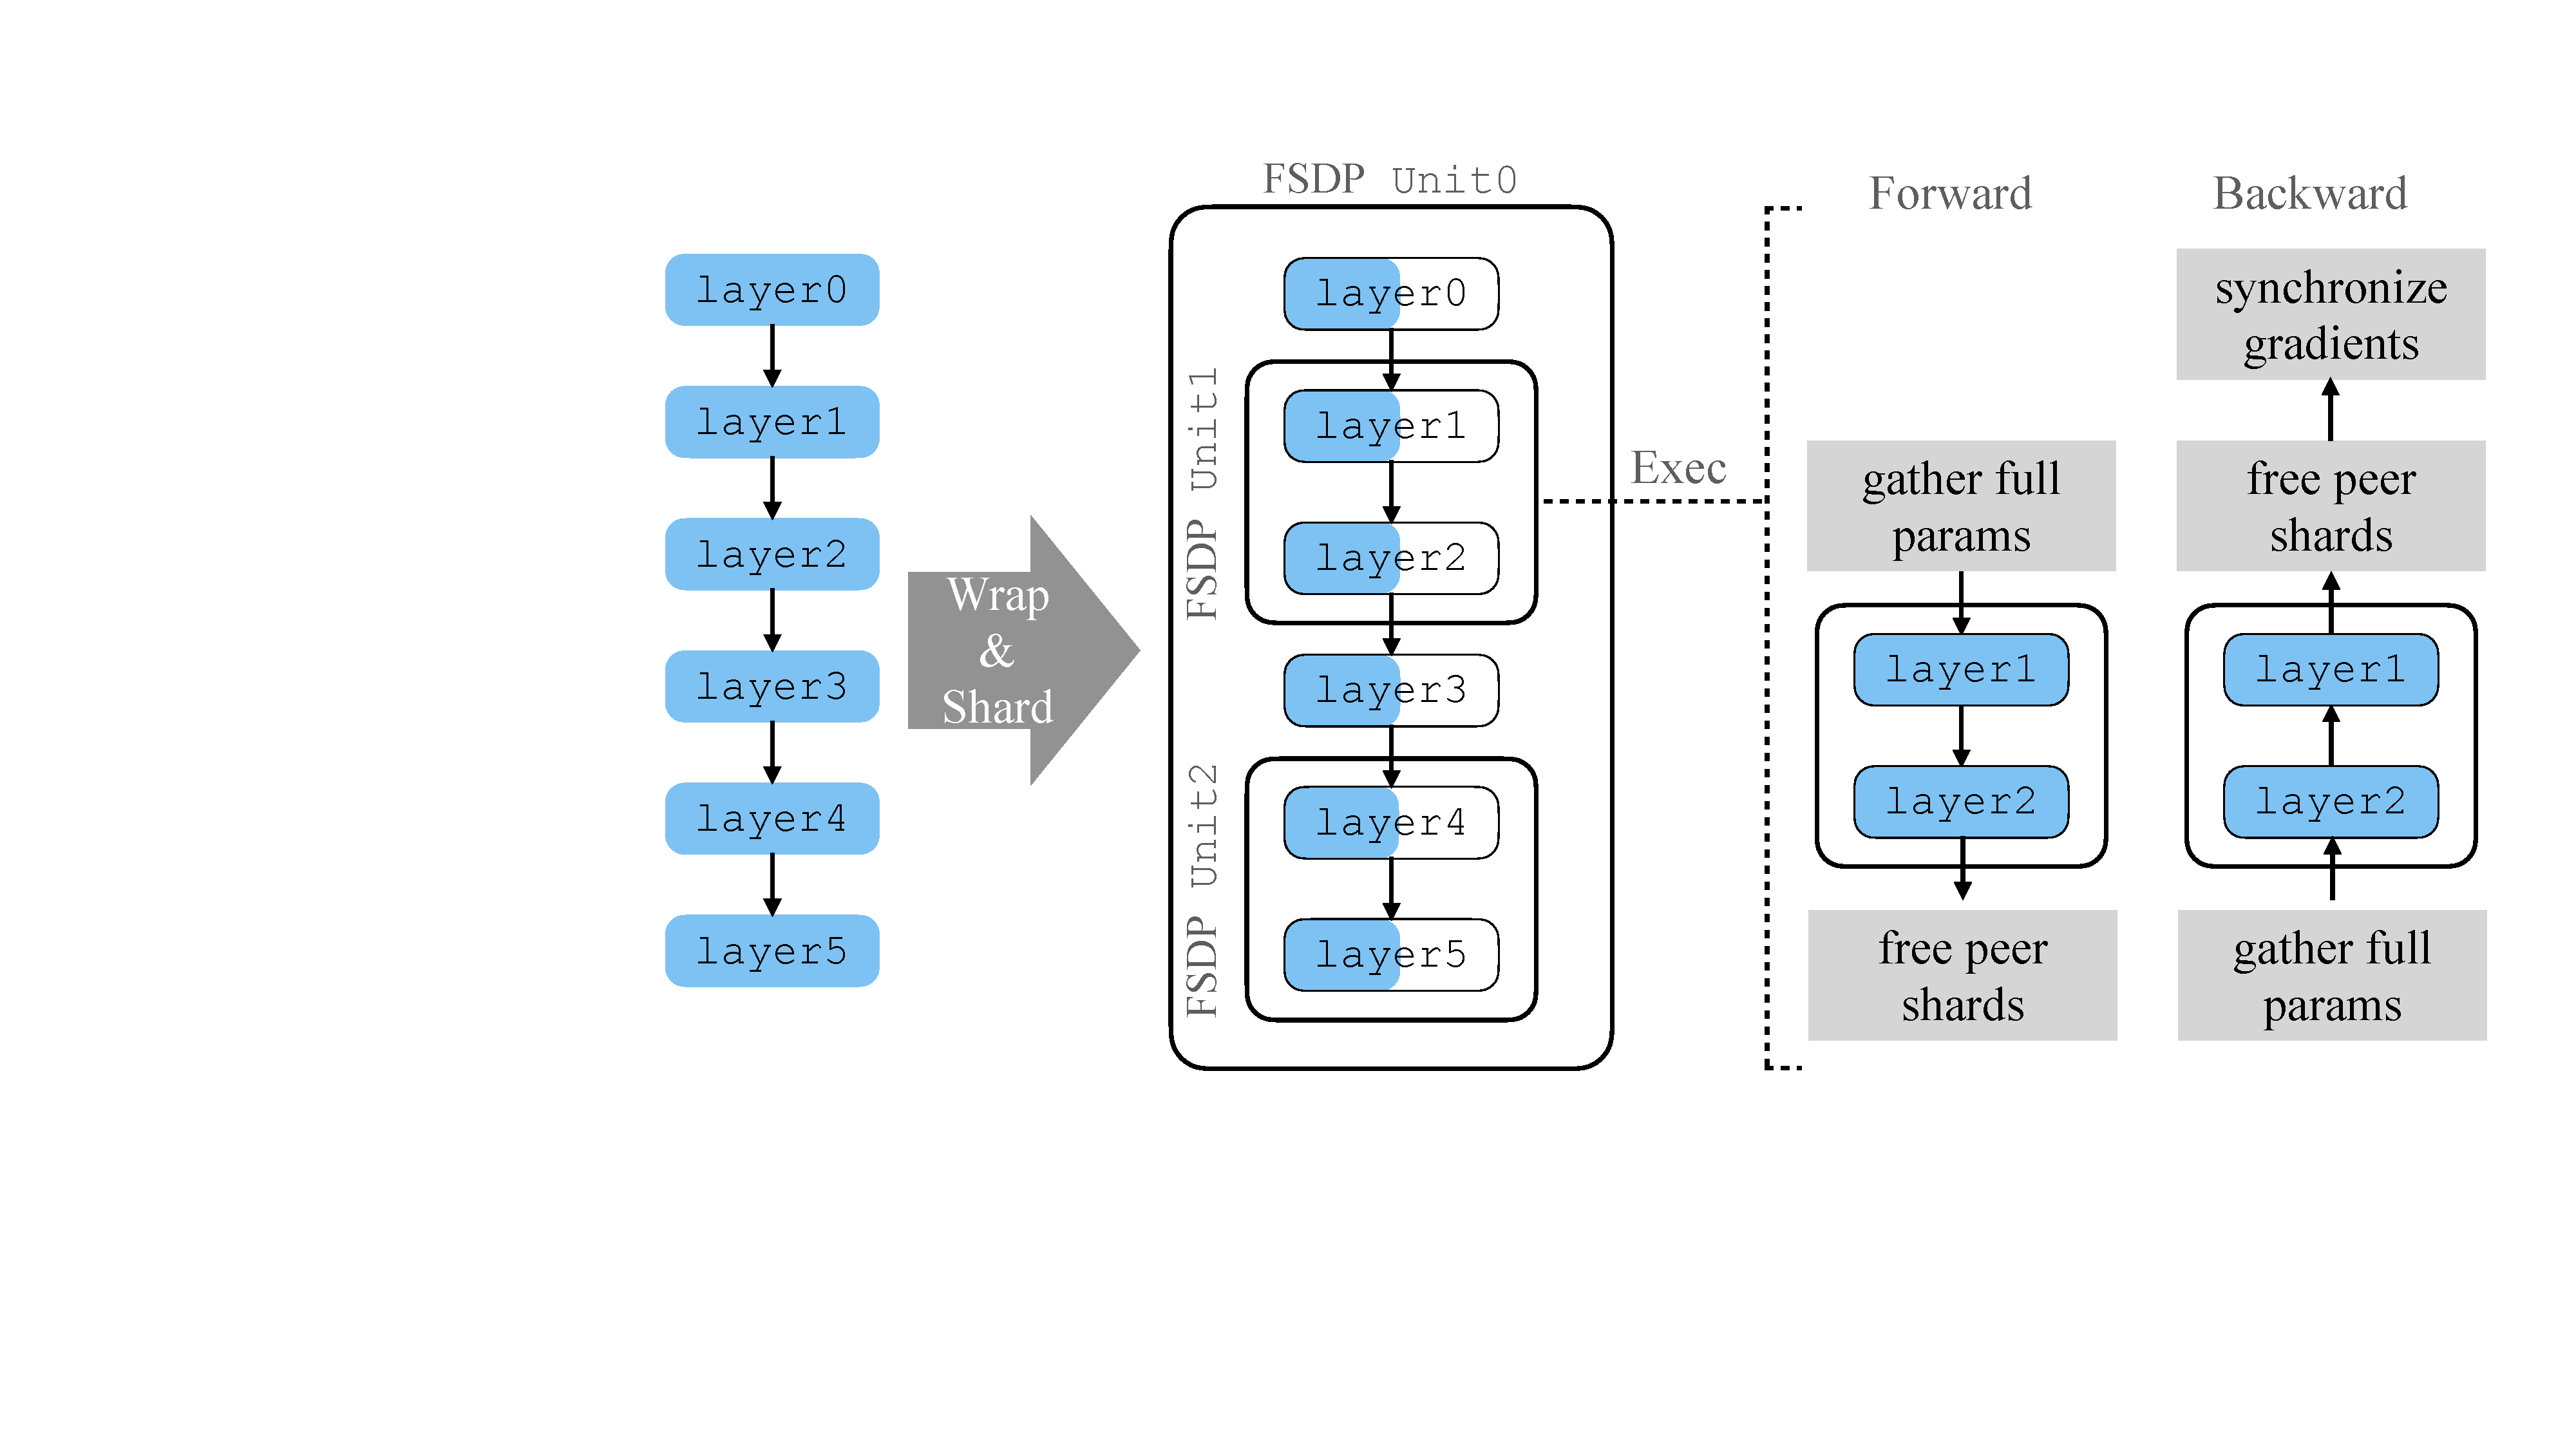
\includegraphics[width=\linewidth]{figure/overview.pdf}
    \caption{FSDP Algorithm Overview}
    \label{fig:overview}
\end{figure}

Figure~\ref{fig:overview} demonstrates the overall workflow using a simple six layer model. Suppose FSDP decomposes the model into three parts, namely, \code{[layer0, layer3]}, \code{[layer1, layer2]}, and \code{[layer4, layer5]}. The decomposition behavior can be controlled by user-defined functions. FSDP then wraps each of these three parts into one FSDP unit and shards parameters accordingly. To ensure correctness, FSDP needs to recover the unsharded parameters before corresponding computations. Let us consider FSDP \code{unit1} that contains \code{[layer1, layer2]} to explain this process. Before forward computation enters \code{layer1}, FSDP collects the unsharded parameters for \code{layer1} and \code{layer2} by gathering shards from other peer ranks. With the unsharded parameters, FSDP runs the local computation of those layers and then frees the peer shards it just collected to reduce memory footprint. Therefore, during the entire forward pass, FSDP only needs to fully materialize one unit at a time, while all other units can stay sharded. Similarly, during the backward computation, FSDP \code{unit1} recovers the unsharded parameters for \code{layer1} and \code{layer2} before backward reaches \code{layer2}. When the autograd engine finishes the backward computation of these two layers, FSDP frees the peer shards and launches \code{ReduceScatter} to reduce and shard gradients. Hence, after backward computation, each rank only keeps a shard of both parameters and gradients. 

FSDP offers a wide spectrum of optimizations and knobs to account for diverse model structures and hardware capabilities. The remainder of this section delves further into the intricacies of model initialization, sharding strategies, communication optimizations, and memory management, which are all critical components of FSDP's underlying design.
